\section{Background}

\begin{frame}[t]{Outline}
\setcounter{tocdepth}{1}
\tableofcontents[currentsection]
\end{frame}

\begin{frame}{Main Challenges}
\begin{itemize}  \itemsep50pt
\item Meaningful and easily correlated tracing data
\item Low overhead tracing backend
\end{itemize}
\end{frame}

\subsection{Tracing concepts}

\begin{frame}{Schools of thought}
\setbeamertemplate{description item}[align left]
\begin{description} \itemsep10pt

\item[black-box schemes] \hfill \\
They assume there is no additional information other than the message record
described above and use statistical regression techniques to infer that
association.

\item[annotation-based schemes] \hfill \\
They rely on applications or middleware to explicitly tag every record with a
global identifier that links these message records back to the originating
request.

\end{description}
\end{frame}

\subsection{Dapper}

\begin{frame}{The Dapper System }

\begin{itemize}
\item Large-scale distributed systems tracing infrastructure created by Google\footfullcite{dapper}
\item Annotation-based tracing scheme
\item Common libraries instrumentation 
    \begin{itemize}
    \item RPC System
    \item Control Flow
    \end{itemize}
\item BigTable backend
\item Closed-source
\end{itemize}
\end{frame}

\begin{frame}{Dapper tracing concepts}
\setbeamertemplate{description item}[align left]
\begin{description}
\item[annotation]
The actual information being logged. Either \emph{timestamp} or \emph{key-value}
\item[span]
The basic unit of the process tree. Can represent a subsystem or a function
call. To depict causal relationship each span has a parent span or is a
\emph{root} span.
\item[trace]
A different trace id is used to group data related to the same initial request
\end{description}
\end{frame}

\begin{frame}{Causal realtionships}
\begin{center}
    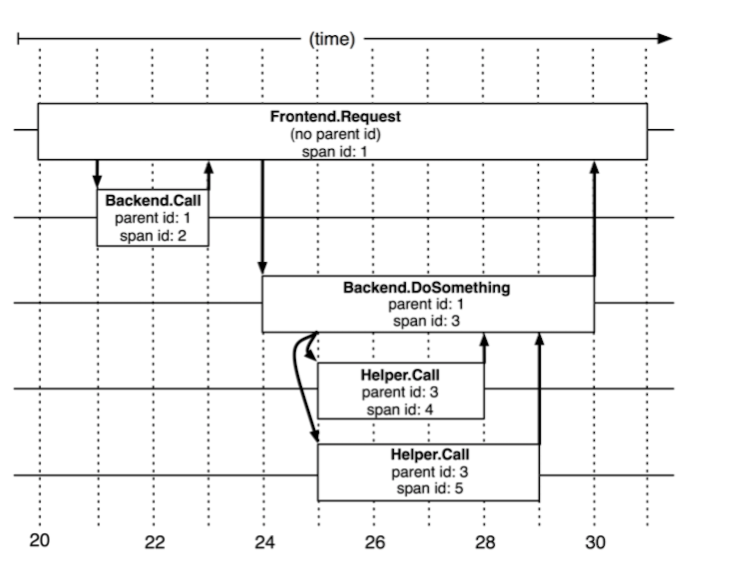
\includegraphics[scale=0.3]{images/dapper.png} \\
\end{center}
\end{frame}
\subsection{Zipkin}

\begin{frame}{Zipkin}
An open-source Scala implementation of the Dapper paper by Twitter
\hfill \\
\hfill \\
Zipkin services:
\begin{itemize}
\item Data collector
\item Database service
\item Web UI
\end{itemize}
\end{frame}

\begin{frame}{Zipkin Architecture}
\begin{center}
    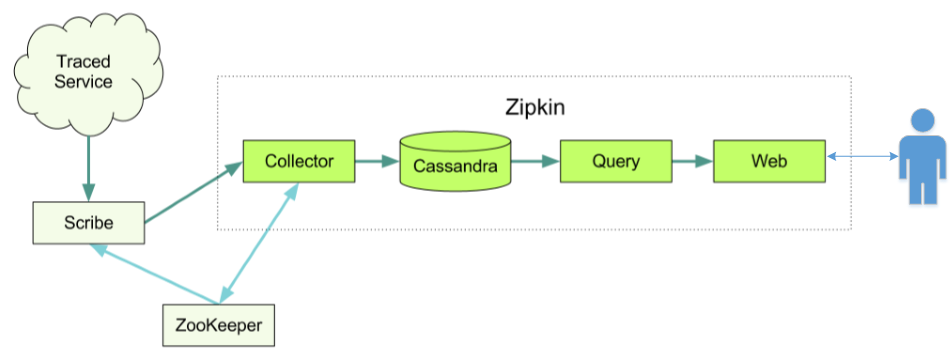
\includegraphics[scale=0.35]{images/zipkin-architecture.png} \\
\end{center}
\end{frame}

\begin{frame}{Scribe}
Scribe is a scalable and reliable logging server created by Facebook
\hfill \\
\hfill \\
\begin{itemize}
\item Written in C++
\item Directed graph architecture
\item Batch messaging
\item HDFS support
\item Based on Apache Thrift
\end{itemize}
\end{frame}

\begin{frame}{Thrift}
A software framework for scalable cross-language services development.
\hfill \\
\hfill \\
Includes a code generation engine to create RPC services across programming
languages based on a Thrift file
\hfill \\
\hfill \\
Sample target languages: C++, Java, Python, PHP, Ruby, Erlang, Perl, Haskell,
OCaml
\end{frame}

\begin{frame}{Zipkin sum up}
\setbeamertemplate{description item}[align left]
\begin{description} \itemsep15pt
\item[Zipkin] is a full-stack tracing system using
\item[Scribe] as its logging server using
\item[Thrift] as its transport protocol
\end{description}
\end{frame}
